\documentclass{article}
\usepackage[utf8]{inputenc}

\title{COSC 419 Assignment 1}
\author{Martin Wallace }
\date{\today}


\usepackage{graphicx} % image library
\graphicspath{ {images/} }
\usepackage{amsmath} % math library
\usepackage{subcaption} % for side-by-side graphics
\usepackage{float} % for side-by-side graphics

\usepackage{listings} % for code snippets
\usepackage{color} % for code snippets
\usepackage{xcolor} % for code snippets
\usepackage{rotating} %for final full page comment, which is rotated sideways

\definecolor{dkgreen}{rgb}{0,0.6,0}
\definecolor{gray}{rgb}{0.5,0.5,0.5}
\definecolor{mauve}{rgb}{0.58,0,0.82}
\newcommand\tab[1][.5cm]{\hspace*{#1}}

% Defines the Java code colors
\lstset{frame=tb,
  language=Java,
  aboveskip=3mm,
  belowskip=3mm,
  showstringspaces=false,
  columns=flexible,
  basicstyle={\small\ttfamily},
  numbers=none,
  numberstyle=\tiny\color{gray},
  keywordstyle=\color{blue},
  commentstyle=\color{dkgreen},
  stringstyle=\color{mauve},
  breaklines=true,
  breakatwhitespace=true,
  tabsize=3
}


\begin{document}
\maketitle
\begin{enumerate}
  \item \textbf{Steps taken per runtime for various sizes of n}
  \\  
  \begin{table}[H]
    \caption{}
    \centering
    \setlength{\tabcolsep}{0.5em} % for the horizontal padding
	{\renewcommand{\arraystretch}{1.2}% for the vertical padding
    \begin{tabular}{| c | r | r | r |}
    \hline
                           & 10     & 100         & 1000 \\
    \hline
    \(\frac{1}{2} n^2\)    &  50.0  &  5000.0     & 500000.0   \\
    \hline
    \(3n \) \(log_2 n\)    &  99.7  & 1993.2      & 29897.4    \\
    \hline
    \(n\sqrt{n}\)          &  31.6  & 1000.0      & 31622.8    \\
    \hline
    \(2^{\frac{n}{4}}\)    &  5.7   & 33554432.0  & 1.8e+75    \\
    \hline
    \end{tabular}
    }
  \end{table}
  
  If the system is expected to support input sizes of ten thousand or more then you would want to use the algorithm with complexity O(\(3n \) \(log_2 n\)).
  
  \item \textbf{An interface for an excel like table }
  \begin{lstlisting}
//Table.java
package assignment1;
import java.io.FileNotFoundException;
public interface Table<T>{
    public void populateFromCSVFile(String csvFilename) throws FileNotFoundException, InvalidCSVException;
    public int height();
    public int width();
    public T[] getRow(int rowNum);
    public T[] getCol(int colNum);
    public T[][] getFullTable();
    public void set(int row, int col, T data);
}
 \end{lstlisting}
 
 \item \textbf{Hashmaps for a shopping list}
 \begin{lstlisting}
package assignment1;

import java.util.HashMap;
import java.util.Map;
import java.util.Scanner;

public class Q3 {
    public static void main(String[] args) {
        /*
            For this question we will assume that the input looks like
            n - Followed by n lines of:
            Item Price
            m - Followed by M lines of:
            Quantity Item
            Assuming that the data is coming from stdin
         */
        Scanner input = new Scanner(System.in);
        Map<String, Double> prices = new HashMap<>();
        double total = 0;
        int n = Integer.parseInt(input.nextLine());
        while(n-->0) {
            String item = input.next();
            double price =  Double.parseDouble(input.nextLine());
            prices.put(item, price);
        }
        int m = Integer.parseInt(input.nextLine());
        while(m-->0) {
            int quantity = Integer.parseInt(input.next());
            String item = input.nextLine().trim();
            if(prices.containsKey(item)) {
                total += prices.get(item) * quantity;
            }else {
                throw new RuntimeException("Undefined grocery item");
            }
        }
        System.out.println(String.format("The total of the shopping list is: $%.2f",  total));
        System.exit(0);
    }
}
 \end{lstlisting}
 The output of running the program:
 \begin{lstlisting}[language=bash]
  $ java Q3 << cat EOF
  5
  Book     8.95
  Pen      0.99
  Eraser   0.50
  Case     3.75
  Backpack 29.99
  4
  1 Backpack
  6 Pen
  2 Eraser
  1 Book
  EOF
  The total of the shopping list is: $45.88
  $
\end{lstlisting}
  
  \item \textbf{Evaluate the run time of a code fragment}
  \\
  \textbf{for} \textit{i} $\leftarrow$ 0 to \textit{n} - 1 \textbf{do} \\
  \tab \textbf{for} j $\leftarrow$ 0 to \textit{n} $\cdot$ \textit{n} - 1 \textbf{do} \\
  \tab \tab  \textbf{for} k $\leftarrow$ 0 to \textit{j} - 1 \textbf{do} \\
  \tab \tab \tab $s \leftarrow s + 1$
  \\
  Given that the outer loop 
  \fcolorbox{lightgray}{lightgray}
  	{\textbf{for} \textit{i} $\leftarrow$ 0 to \textit{n} - 1 \textbf{do}
  }
  will  run exactly \textit{n} times we know that the each piece of code inside this loop will run exactly \textit{n} times. Therefor we can say that the run time of the entire expression is O(n) $\cdot$ O(inner loops).
  \\
  \\
  Given that the first inner loop 
  \fcolorbox{lightgray}{lightgray}
  	{\textbf{for} j $\leftarrow$ 0 to \textit{n} $\cdot$ \textit{n} - 1 \textbf{do}
  }
  will run exactly $n^2$ times we can say that the run time of the entire expression is O(n) $\cdot$ O($n^2$) $\cdot$ O(inner loop).
  
 Given that the last inner loop
 \fcolorbox{lightgray}{lightgray}
   {\textbf{for} k $\leftarrow$ 0 to \textit{j} - 1 \textbf{do}
 }
 will run on average $\frac{1}{2}n^2$ times. 
 \\
 \\
 Then we can say that the run time of the entire code fragment is O(n) $\cdot$ O($n^2$) $\cdot$ O($\frac{1}{2}n^2$), or  O($n^5$). 
 
 \item \textbf{The evil (and cheap) king}
 \\
 Given that the king has \textit{n} bottles of wine, only 1 bottle is poisoned, and it will take exactly one month to kill anyone who drinks a drop of wine, we can determine which glass of wine was poisoned in one month using exactly ceil(\textit{$log_2$\textit{n}}) taste testers. 
 \begin{enumerate}
 	\item First label each bottle from \textit{1..n} with numbers \textit{0..n-1} respectively.
 	\item Set $m \leftarrow ceil(log_2\textit{n})$.
 	\item Next gather your \textit{m} taste testers and brand them (literally, because you are an evil king) with a number from \textit{0..m-1}.
 	\item Now for each bottle with number \textit{i} we will have each taste tester with   a number \textit{j}, such that $(1 << j)$ $\&$ $i = 1$, drink a drop from the bottle.
 	Or less formally \textit{j} is the index of a bit which is set to 1 in the binary representation of \textit{i}. 
	\item One month later gather of all of taste testers who died and put their numbers into set D. Now the number on the label of the poisoned bottle of wine is equal to $$\sum_{j \in D} 2^j$$
 \end{enumerate}
 	For example, if testers with numbers 0, 1 and 2 assigned to them died, we would know that the poisoned bottle was bottle number 7 ($2^0 +  2^1 + 2^2)$. However, if taste tester number 3 died instead of number 0, then we would know that the number of the poisoned bottle would be 14 ($2^1 + 2^2 + 2^3$).

 
 \item 
 \textbf{Skip Lists}
 \\
 The results of inserting 12, 20, 40 with the next 12 flips being HTHHTHTHTTHH
 \\
 \begin{figure}[H]
 	\centering
 	\caption{Final Result of Skip List}
 	\label{fig:SkipList}
	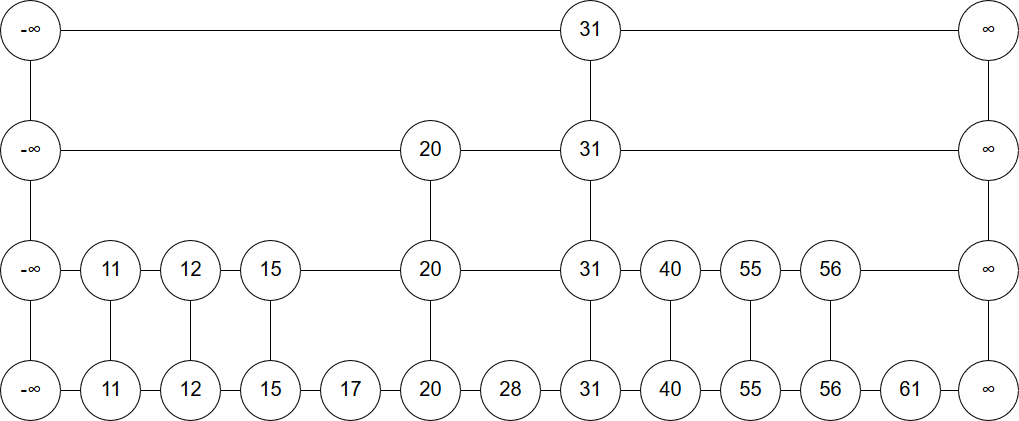
\includegraphics[width=\textwidth]{SkipList}
 \end{figure}
 
 \item \textbf{Heaps}
 \\
 Vladimir is wrong that a preorder traversal will always list its keys in non-decreasing order. For example in the figure below, the preorder traversal would be 1,2,4,5,3. Since 5 $>$ 3 this breaks the nondecreasing order that Vladimir claims.
 
  \begin{figure}[H]
 	\centering
 	\caption{A heap that breaks Vladimir's assumptions}
 	\label{Heaps}
	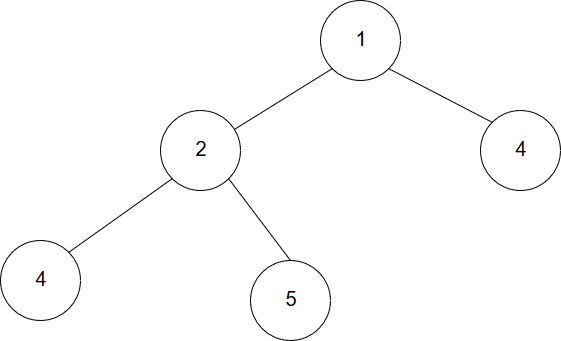
\includegraphics[width=\textwidth]{Heap}
 \end{figure}
 

 \item \textbf{Search Trees}
 \\
 Margherita is wrong that the order of insertion into a binary tree does not matter. As seem below.

  \begin{figure}[H]
    \centering
    \begin{subfigure}{.5\textwidth}
      \centering
      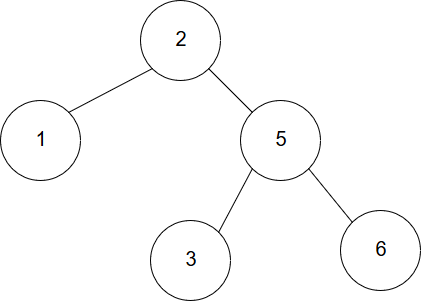
\includegraphics[width=.98\linewidth]{BinaryTree1}
      \caption{The result of inserting 2,5,1,6,3}
      \label{fig:BinaryTree:sub1}
    \end{subfigure}%
    \begin{subfigure}{.5\textwidth}
      \centering
      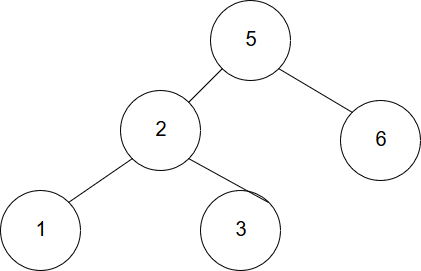
\includegraphics[width=.98\linewidth]{BinaryTree2}
      \caption{The result of inserting 5,2,3,1,6}
      \label{fig:BinaryTree:sub2}
    \end{subfigure}
    \caption{Two distinct binary trees with the same set of keys}
    \label{fig:BinaryTree}
  \end{figure}

  \item \textbf{Ternary Trees}
  	\begin{enumerate}
  		\item Given that a full ternary tree with depth 0 has 1 node, depth 1 has 4 nodes and depth 2 has 13 nodes. We can see that each level of depth \textit{f} has exactly $3^\textit{f}$ nodes at that level. So a full tree of depth \textit{d} would have $$\sum_{i=0}^{d} 3^i $$ nodes. This can be written in the closed form of $$\frac{3^{d+1} - 1}{2}$$
  		\item Given that the tree is zero-indexed, we can find the left, centre and right children of any given index using the following three formulas:
  		\begin{itemize}
  			\item $left(i)  \rightarrow i \cdot 3 + 1$
  			\item $centre(i) \rightarrow i \cdot 3 + 2$
  			\item $right(i) \rightarrow i \cdot 3 + 3$
  		\end{itemize}
  		\item $depth(i) \rightarrow floor(log_3 ((i + 1)*2))$ 
  		\\
  		
  	\end{enumerate}
 
 \item \textbf{Search Trees}
 	\\	
 	Show the results of inserting 15,6,12,1,14,11,4,13,3,9,10,2,5,7,8 in the given order into various trees.
 	
 	\begin{figure}[H]
 	  \centering
 	  \caption{Items inserted into a binary tree}
 	  \label{Trees:BinaryTree}
	  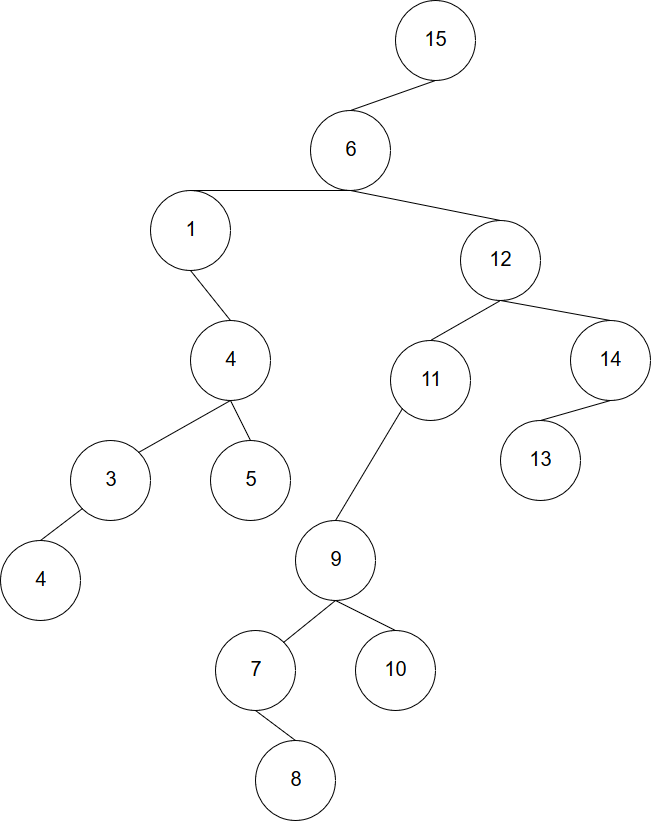
\includegraphics[width=\textwidth]{BinaryTree3}
    \end{figure}
      
    \begin{figure}[H]
 	  \centering
 	  \caption{Items inserted into a red black tree}
 	  \label{Trees:RedBlackTree}
	  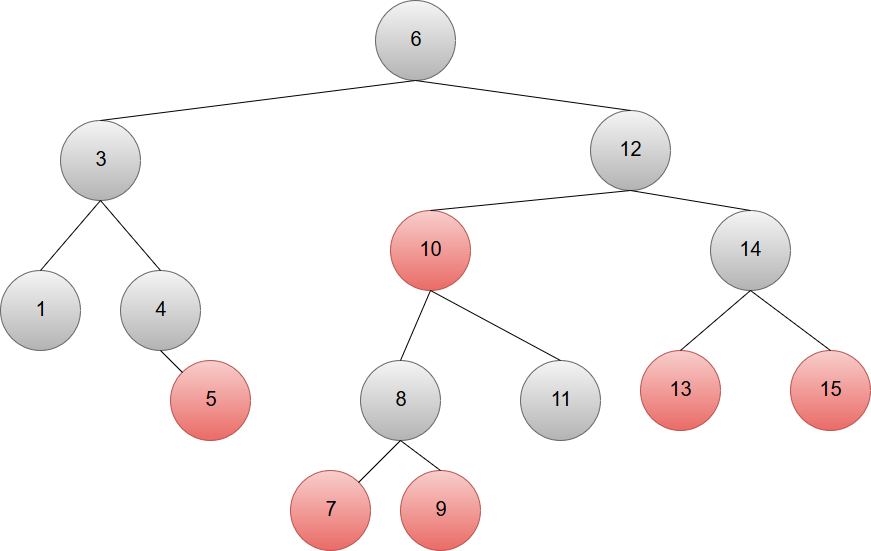
\includegraphics[width=\textwidth]{RedBlackTree}
    \end{figure}

	\begin{figure}[H]
 	  \centering
 	  \caption{Items inserted into a splay tree}
 	  \label{Trees:SplayTree}
	  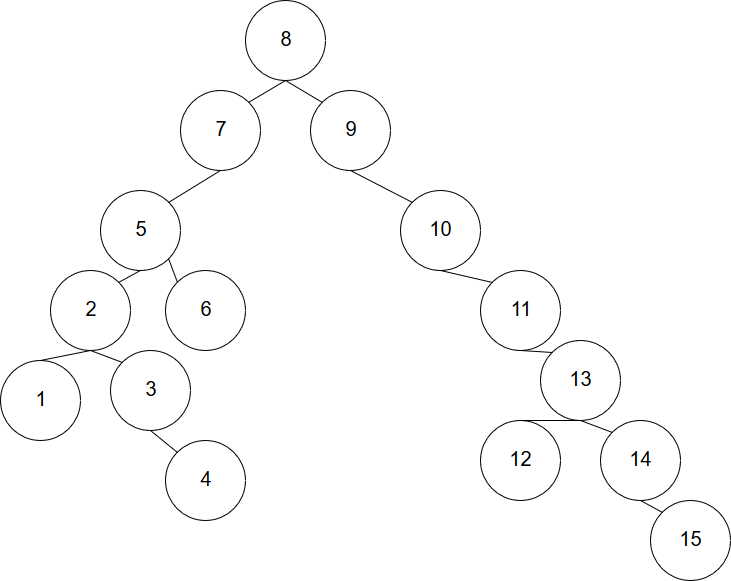
\includegraphics[width=\textwidth]{SplayTree}
    \end{figure}
    
    \begin{figure}[H]
 	  \centering
 	  \caption{Items inserted into a 2-4 tree}
 	  \label{Trees:24Tree}
	  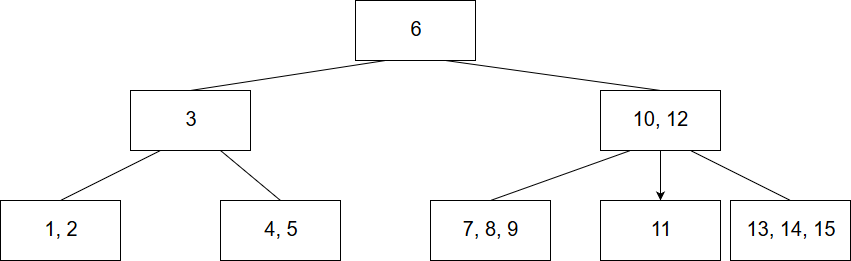
\includegraphics[width=\textwidth]{2-4}
    \end{figure}
    
    Show the results after each step of removing 5,8,6 for each tree
    
    \begin{figure}[H]
 	  \centering
 	  \caption{Binary tree after removing 5}
 	  \label{Trees:BinaryTreeR1}
	  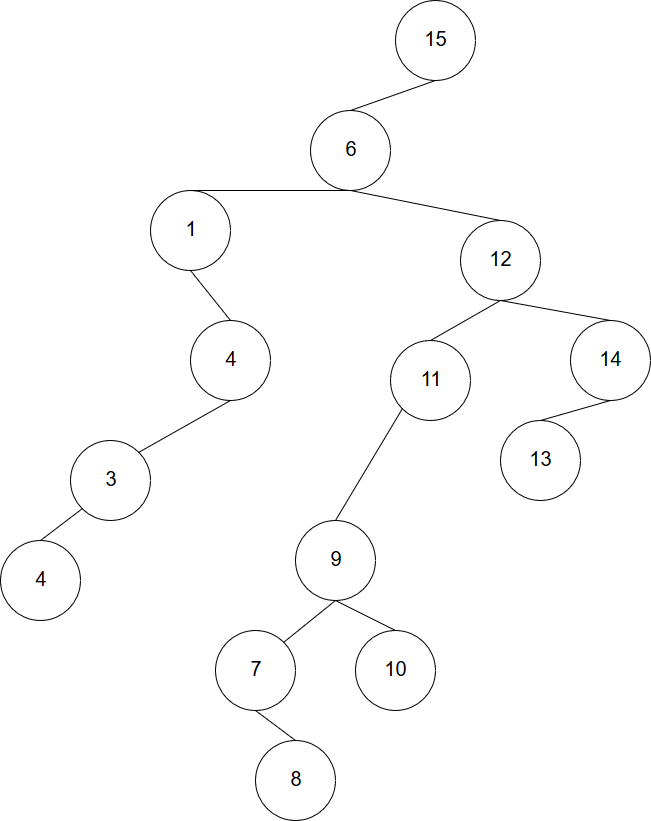
\includegraphics[width=\textwidth]{BinaryR1}
    \end{figure}
    \begin{figure}[H]
 	  \centering
 	  \caption{Binary tree after removing 8}
 	  \label{Trees:BinaryTreeR2}
	  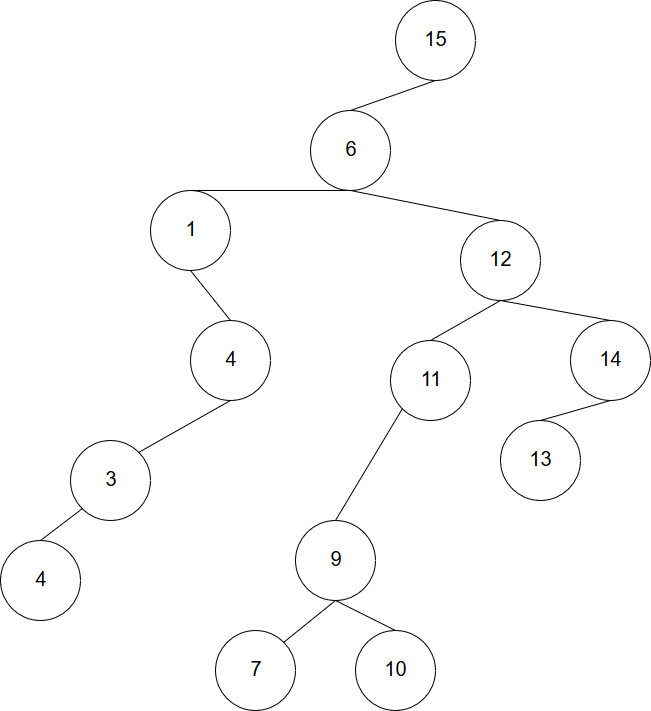
\includegraphics[width=\textwidth]{BinaryR2}
    \end{figure}
    \begin{figure}[H]
 	  \centering
 	  \caption{Binary tree after removing 6}
 	  \label{Trees:BinaryTreeR3}
	  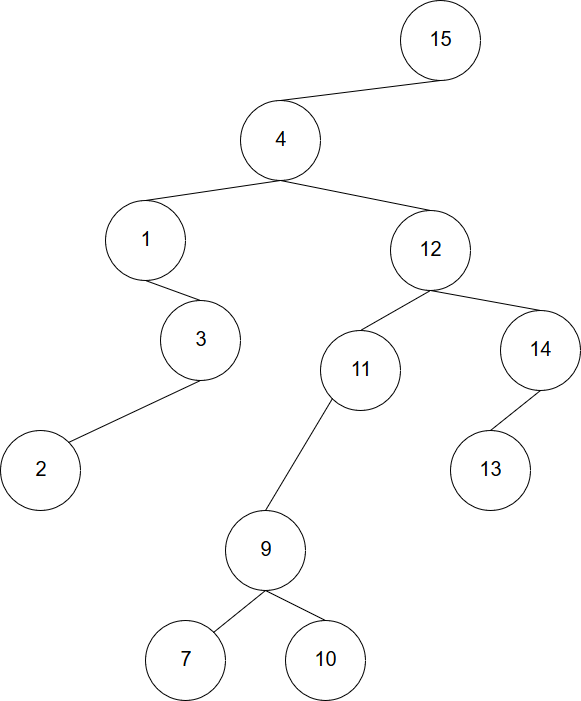
\includegraphics[width=\textwidth]{BinaryR3}
    \end{figure}
    
    \begin{figure}[H]
 	  \centering
 	  \caption{Red black tree after removing 5}
 	  \label{Trees:RedBlackR1}
	  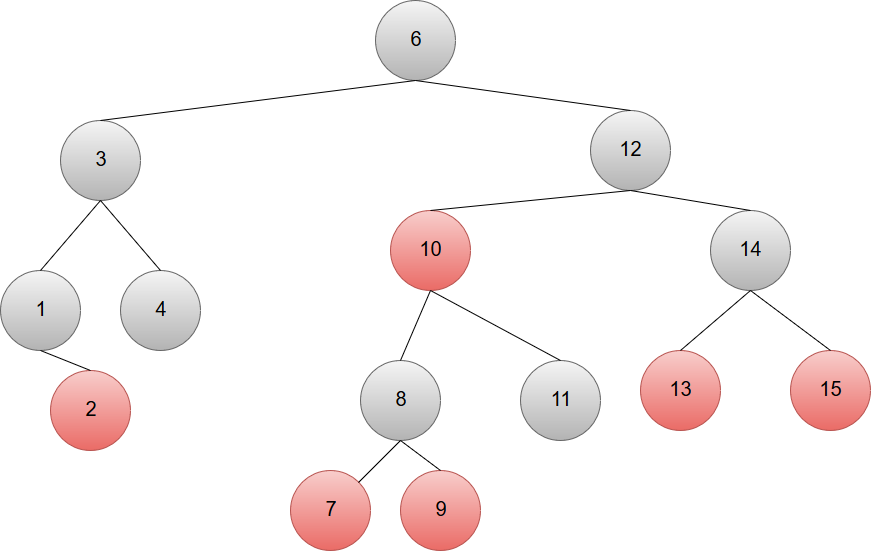
\includegraphics[width=\textwidth]{RedBlackR1}
    \end{figure}
    \begin{figure}[H]
 	  \centering
 	  \caption{Red black tree after removing 8}
 	  \label{Trees:RedBlackR2}
	  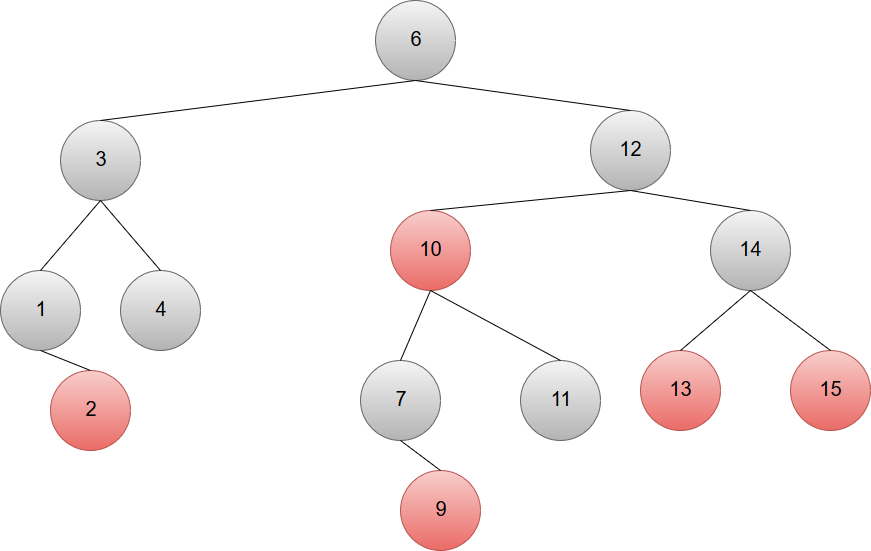
\includegraphics[width=\textwidth]{RedBlackR2}
    \end{figure}
    \begin{figure}[H]
 	  \centering
 	  \caption{Red black tree after removing 6}
 	  \label{Trees:RedBlackR3}
	  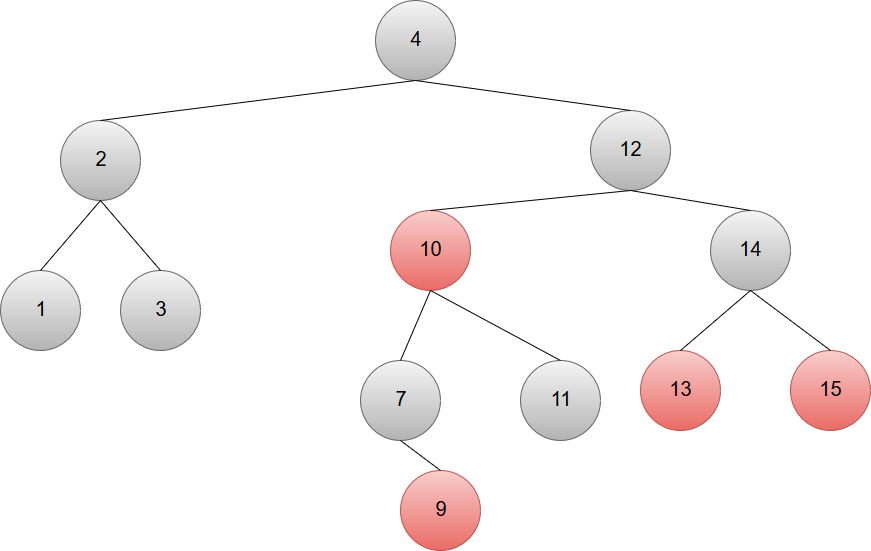
\includegraphics[width=\textwidth]{RedBlackR3}
    \end{figure}
    
    
    \begin{figure}[H]
 	  \centering
 	  \caption{Splay tree after removing 5}
 	  \label{Trees:SplayR1}
	  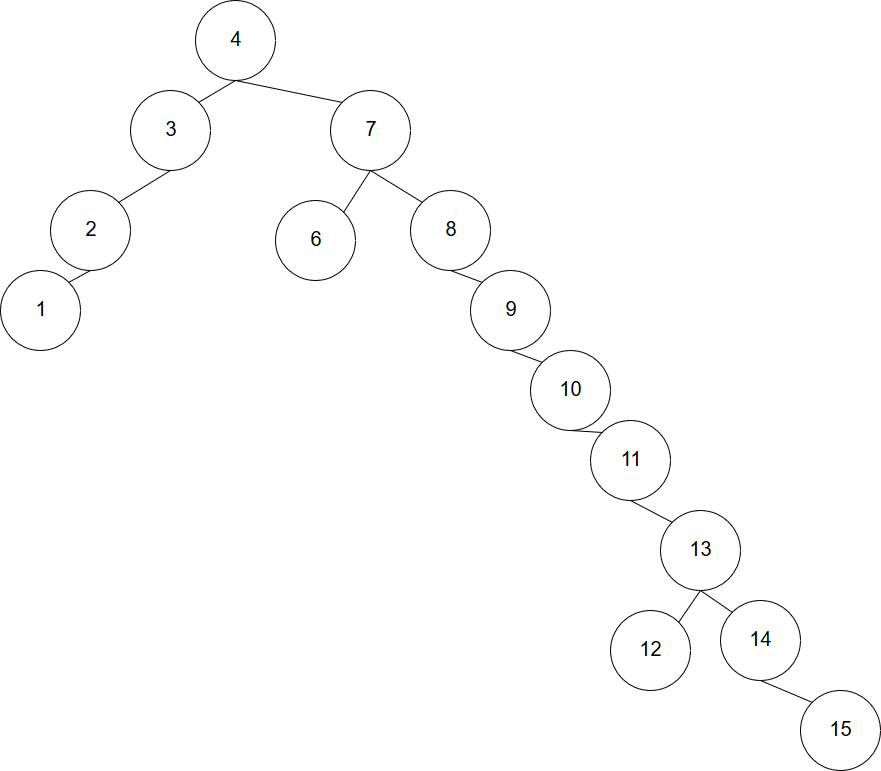
\includegraphics[width=\textwidth]{SplayR1}
    \end{figure}
    \begin{figure}[H]
 	  \centering
 	  \caption{Splay tree after removing 8}
 	  \label{Trees:SplayR2}
	  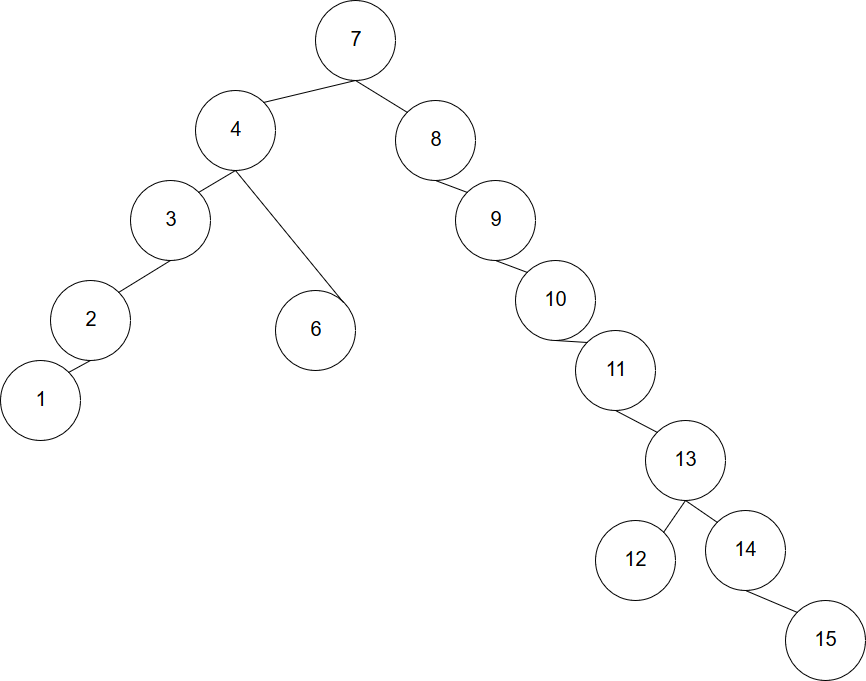
\includegraphics[width=\textwidth]{SplayR2}
    \end{figure}
    \begin{figure}[H]
 	  \centering
 	  \caption{Splay tree after removing 6}
 	  \label{Trees:SplayR3}
	  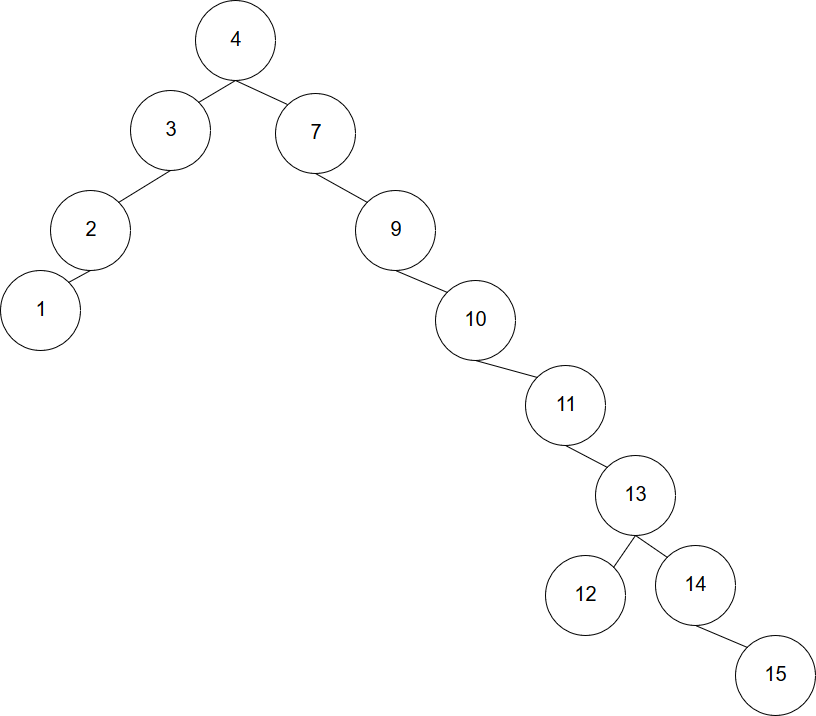
\includegraphics[width=\textwidth]{SplayR3}
    \end{figure}
    
    \begin{figure}[H]
 	  \centering
 	  \caption{2-4 tree after removing 5}
 	  \label{Trees:2-4R1}
	  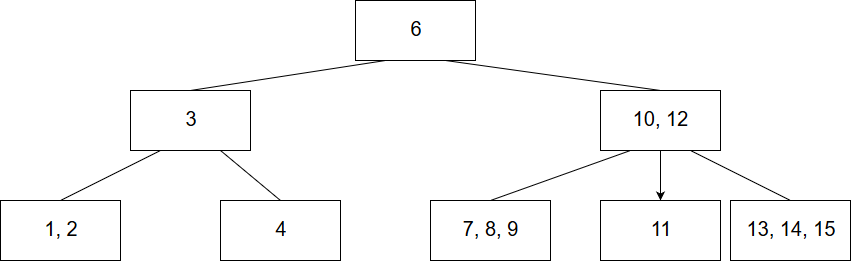
\includegraphics[width=\textwidth]{2-4R1}
    \end{figure}
    \begin{figure}[H]
 	  \centering
 	  \caption{Splay tree after removing 8}
 	  \label{Trees:2-4R2}
	  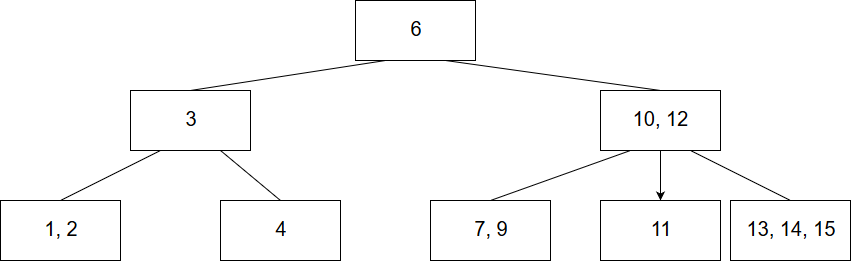
\includegraphics[width=\textwidth]{2-4R2}
    \end{figure}
    \begin{figure}[H]
 	  \centering
 	  \caption{Splay tree after removing 6}
 	  \label{Trees:2-4R3}
	  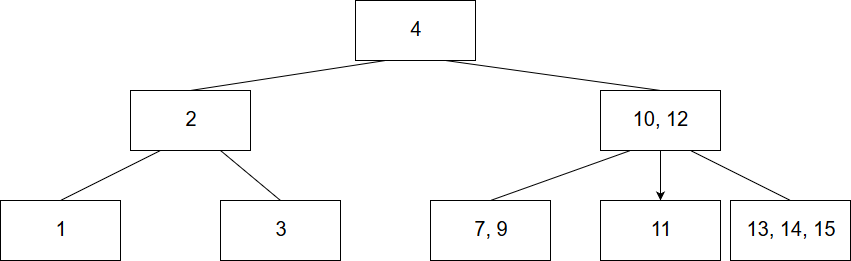
\includegraphics[width=\textwidth]{2-4R3}
    \end{figure}
    
  \item \textbf{2-3 Tree}
  \\
  Show the results of inserting 15,6,12,1,14,11,4,13,3,9,10,2,5,7,8 into a 2-3 Tree
  	\begin{figure}[H]
 	  \centering
 	  \caption{2-3 Tree after inserts}
 	  \label{Trees:2-3Tree}
	  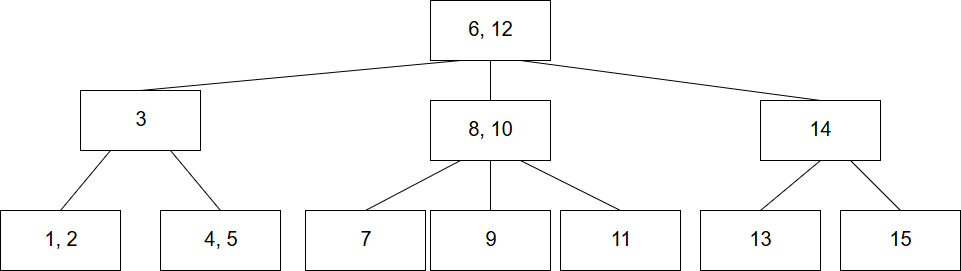
\includegraphics[width=\textwidth]{2-3Tree}
    \end{figure}
  
  \item \textbf{Huffman Code}
  \begin{enumerate}
  	\item The given text contains 1289 characters, which means that if we needed 7 bytes to for each character we would require a total of 9023 bytes. 
  	\item 
  	
  	Full Huffman Tree (larger version available at end of document)
  	\begin{figure}[H]
 	  \centering
 	  \caption{2-3 Tree after inserts}
 	  \label{Trees:2-3Tree}
	  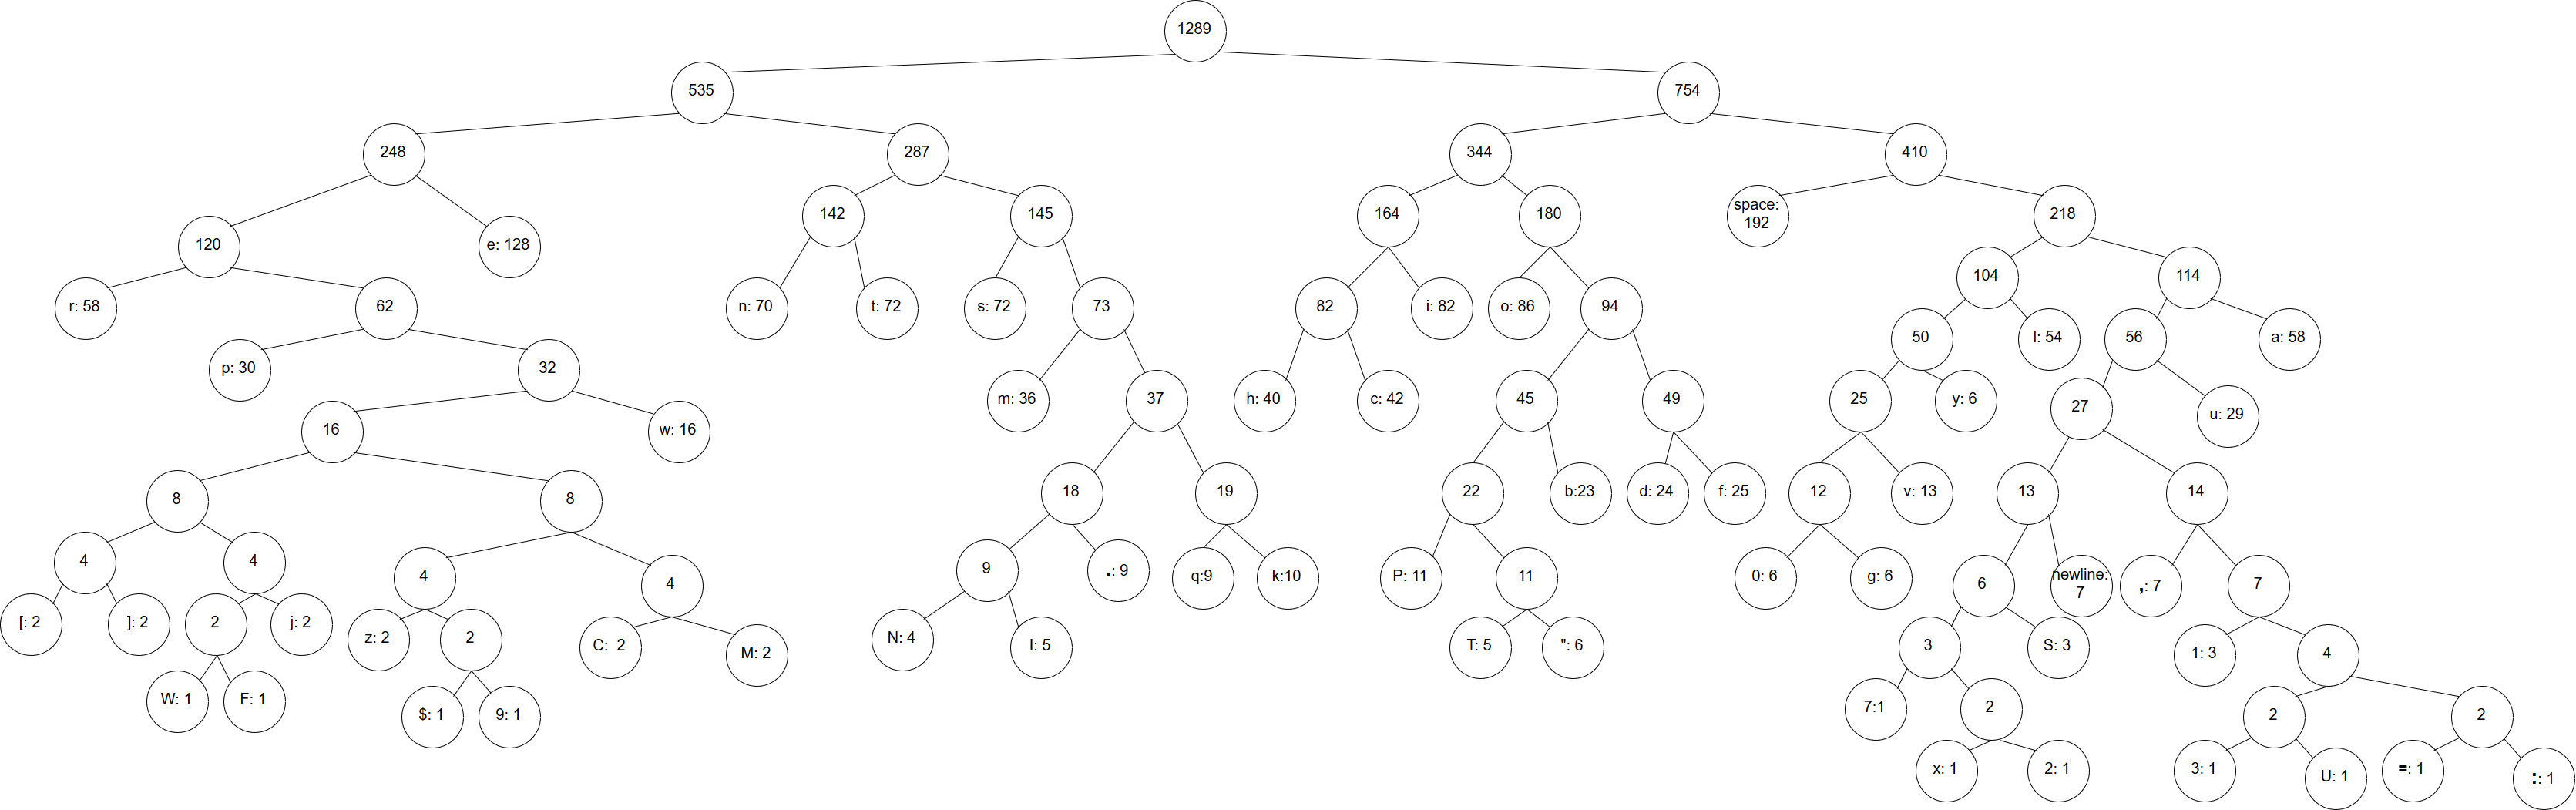
\includegraphics[width=\textwidth]{Huffman}
    \end{figure}
  	\item The number of bits required to store the text in a prefix code was 5882 which is only 65.2\% of the number of bits required for the uncompressed version. 
  
  \end{enumerate}
  
  
  \item \textbf{Pattern Matching}
    \begin{figure}[H]
 	  \centering
 	  \caption{Boyer Moore Algorithm searching for  amanpa in amanaplanacanalpanama}
 	  \label{Trees:BoyerMoore}
	  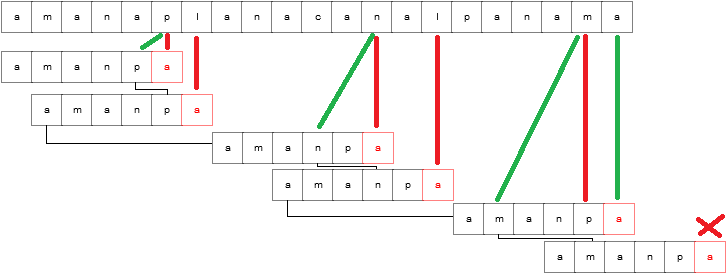
\includegraphics[width=\textwidth]{BoyerMoore}
    \end{figure}
 
  \item \textbf{Tries}
    \begin{figure}[H]
 	  \centering
 	  \caption{The compressed suffix trie of RETREATER}
 	  \label{Trees:CompressedSuffixTrie}
	  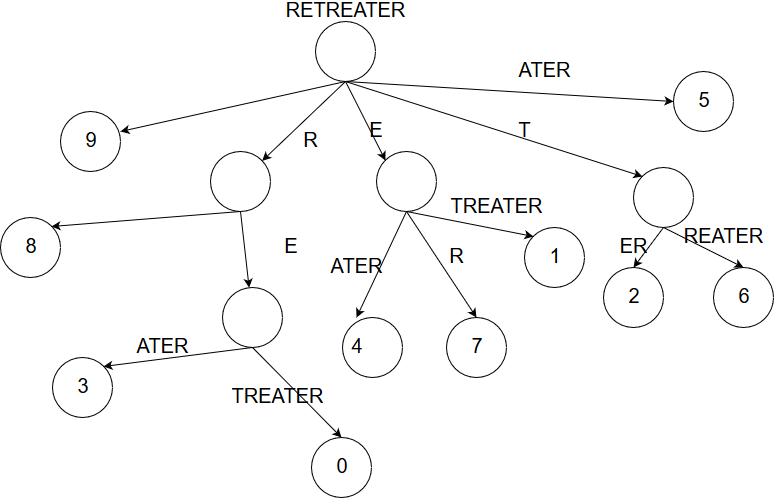
\includegraphics[width=\textwidth]{CompressedSuffixTrie}
    \end{figure}
  
  \item \textbf{2-4 Tree Contains Method}

  \begin{lstlisting}
  
package assignment1;
public class TwoFourTree {
    static class Node {
        int size;
        int[] keys = new int[3];
        Node[] children = new Node[4];
    }
    public static boolean find(Node r, int k) {
        // Make sure node is valid
        if (r == null ||  r.size == 0)
            return false;
        for(int i = 0; i < r.size; i++)
            if(k == r.keys[i])
                return true;
            else if(k < r.keys[i])
                return find(r.children[i], k);
        // If we made it here then k > all keys 
        // call find on rightmost child
        return find(r.children[r.size], k);
    }
}
 \end{lstlisting}
  
  
\end{enumerate}


\begin{sidewaysfigure}
  \centering
  \caption{2-3 Tree after inserts}
  \label{Trees:2-3Tree}
  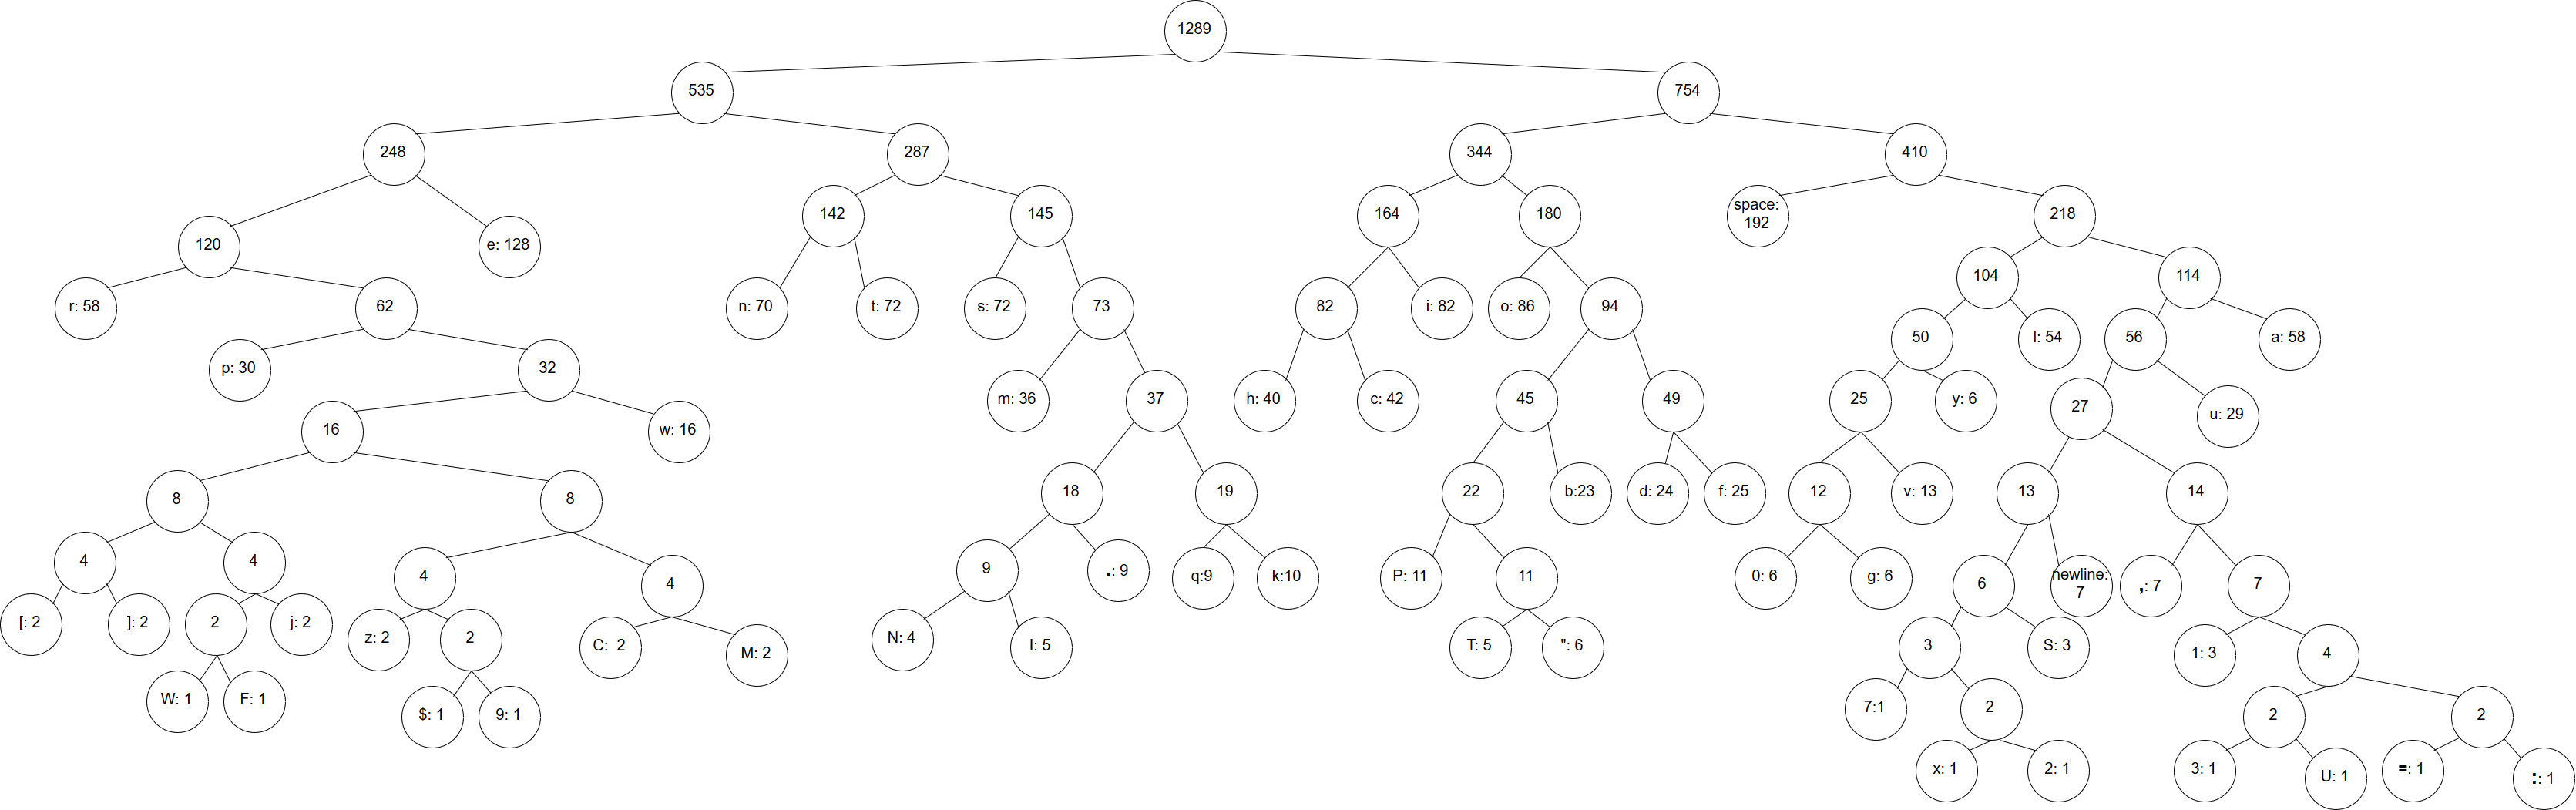
\includegraphics[width=\paperwidth]{Huffman}
\end{sidewaysfigure}

\end{document}
